\documentclass[11pt]{article}
\usepackage{acl2014}
\usepackage{times}
\usepackage{url}
\usepackage{graphicx}
%\usepackage{latexsym}


%figures:
\usepackage{tikz}
\usetikzlibrary{trees,positioning,backgrounds}
%\usepackage{tikz-qtree}
\usepackage{subcaption}

%references and keeping floats in place
\usepackage[pdftex,pdfborder={0 0 0},unicode,breaklinks,hyperfootnotes=false,bookmarks]{hyperref}
\usepackage[section]{placeins}

\usepackage{amsmath} 
\renewcommand{\vec}[1]{\mathbf{#1}}

\title{Statistical Structure in Language Processing \\ IBM Model 1}
\author{ Cristina G\^arbacea\\
  10407936 \\
  {\small \tt cr1st1na.garbacea@gmail.com} 
  \\\And
  Sara Veldhoen \\
10545298   \\
  {\small \tt sara.veldhoen@student.uva.nl} \\}

\date{}

\begin{document}

\maketitle

\begin{abstract}
In this paper we present the theoretical notions underlying the IBM Model 1 we implemented and the Expectation Maximization algorithm we applied to train the given parallel Dutch - English corpus. 
%We show that this model can easily overfit and that maximizing the likelihood of the training data can result in low performance accuracy.% Do we?
We also came up with our own extension to the model, which we compare and evaluate against the basic IBM model 1. 
\end{abstract}

\section{Introduction}
%Statistical alignment models are widely used nowadays in a variety of natural language processing applications, ranging from machine translation to question answering and information retrieval. 
The goal of finding the best English translation $\vec{e}$ of a foreign sentence $\vec{f}$ is modeled under the assumption of the \textit{noisy channel} hypothesis, which considers the foreign sentence as a ``corrupted" instance of the original English sentence. The English sentence which is at the source of its foreign counterpart is an unknown issue, and thus the task of translating $\vec{f}$ into $\vec{e}$ becomes one of maximizing the probability of the English sentence given the foreign sentence, $P(\vec{e}|\vec{f})$. According to Bayes' theorem, 
%
%\begin{equation}
%P(\vec{e}|\vec{f})= \frac{P(\vec{e})\cdot P(\vec{f}|\vec{e})}{P(\vec{f})}
%\end{equation}
%
the translation problem can be expressed as:
\begin{equation}
P(\vec{e}|\vec{f})= arg \ \underset{\vec{e}}{max} \ P(\vec{e})\cdot P(\vec{f}|\vec{e})
\end{equation}

where $P(\vec{e})$ denotes the language model, that takes care of the fluency of the output, 
 and $P(\vec{e}|\vec{f})$ denotes the translation model, that makes sure the translation is adequate. 

In order to be able to approximate this probability, we need to make assumptions. In %cite IBM paper
\cite{Koehn:2010}, \cite{Brown:2010} a series of increasingly complex models is presented. We implemented the first model, hereafter IBM model~1. 

In what follows we present this model in section~\ref{IBM1}, together with the Expectation Maximization formula used for training this model. We came up with an improvement over this model, which we introduce in section~\ref{Improvement}. Then comes an evaluation of the alignment quality for both models in section~\ref{Eval} and finally we conclude in Section~\ref{Concl}.




\section{IBM Model 1}
\label{IBM1}

The assumption underlying the IBM models is that translating text comes down to aligning the words 
%IBM models focus on the translation task only which assumes that word alignments exist between the words 
of the foreign and the English sentence, and translating the words independently.
The words of the English sentence $\vec{e}$ are called \textit{cepts} and generally within the IBM models groups of  words in the foreign sentence $\vec{f}$ cannot be aligned to groups of cepts.  Rather, each foreign word  is aligned to one cept or, in case there is no English correspondent, to the so called \textit{null} word.
Because of this simplification, an alignment can be represented as a vector $\vec{a}$ that has the same length as the foreign sentence: $m$.

The translation probability $P(\vec{f}|\vec{e})$ can be rewritten as the sum over all possible alignments $\vec{a}$ of conditional probabilities $P(\vec{f}, \vec{a}|\vec{e})$:
\begin{align}
P(\vec{f}|\vec{e}) =& \sum_\vec{a} P(\vec{f},\vec{a}|\vec{e})\notag\\
=&\sum_\vec{a}  P(\vec{f},\vec{a},m|\vec{e}) \notag\\
=&\sum_\vec{a}  P(m|\vec{e})\times P(\vec{f}|\vec{a},m,\vec{e})\notag\\
=&  P(m|\vec{e}) \sum_\vec{a} P(\vec{f}|\vec{a},m,\vec{e})\\
P(\vec{f}|\vec{a},m,\vec{e})=&\prod_{j=1}^{m} P(a_j|a_1^{j-1}, f_1^{j-1}, m, \vec{e}) \notag \\
& \times  P(f_j|a_1^j,f_1^{j-1},m,\vec{e})\label{p(f|a,m,e)}
\end{align}


%IBM models build upon one another in increasing order of complexity. IBM Model 1 is the simplest probabilistic generative model based on lexical translation which assumes a word-to-word mapping between the target and the source sentence. It is widely used in working with parallel bilingual corpora, aligning syntactic fragments and estimating phrase translation probabilities.

%The translation probability of a foreign sentence $\vec{f}$ of length $m$ into an English sentence $\vec{e}$ of length $l$ that is aligned as $\vec{a}$ is defined as:
%\begin{equation}p(\vec{e},\vec{a}|\vec{f}) = \frac{\epsilon}{(l + 1)^m} \prod_{j=1}^{m}t(e_j|f(a_j))\end{equation}

%Did the languages change position here? We were estimating p(f,a|e)

\paragraph{EM Training}
The input to the training is a corpus of paired sentences.
To estimate the latent variables, alignments, a version of expectation maximization is used.
Training focuses on the parameters in equation \ref{p(f|a,m,e)}. The first term, the alignment probability, is assumed to be uniform in IBM Model 1.

The initial step of EM consists in setting uniform translation probabilities $t(e|f)$ over the target vocabulary. 

In the E-step, the alignment probabilities are computed. Note that this is done implicitly, in the process of gathering the fractional counts:
\begin{align}
c(f|e;\vec{f},\vec{e}) =& 
\frac{t(f|e)}{t(f|e_0)+\ldots+t(f|e_l)} \notag\\
&\times \sum_{j=1}^m \delta(f,f_j) \sum_{i=0}^l \delta(e,e_i)
\end{align}

The translation probabilities are re-estimated in the M-Step, using the obtained counts:
\begin{align}
t(f|e) = \lambda_e^{-1} \sum_{s=1}^S c(f|e;\vec{f}^{(s)},\vec{e}^{(s)})\\ 
\lambda_e = \sum_f\sum_{s=1}^S c(f|e;\vec{f}^{(s)},\vec{e}^{(s)}) \label{normalization}
\end{align}
Where equation \ref{normalization} ($\lambda_e$) defines the normalization parameter to get proper probabilities.


\section{Improvement Over IBM Model 1}
\label{Improvement}

In IBM Model 1, all alignments are equally probable. The Viterbi alignment can thus be found by simply choosing, for each word, the cept that has the highest translation probability. 

An improvement can be made by introducing a probability function over alignments: the first term in equation \ref{p(f|a,m,e)}.
For simplification, we assume independence of each alignment decision, and independence of lexical items, such that we can compute $p(a_j|j,m,l)$ for each word.

This is also done in IBM Model 2. However,  instead of training the alignment probabilities, as in IBM Model 2, we use a heuristic function. We base this function on the assumption that a word in the input should stay close, i.e. we want to favor $a_j=j$ over $a_j>j$ and $a_j<j$. Furthermore, we tried to favor choosing the null word as presented in \cite{Moore:2004}, but that resulted in a drop in performance. The alignment function we created is defined as 
\begin{equation}
p(a_j|j,m) = \frac{1}{m+|a_j-j|}
\end{equation}

\section{Experiments and Results}
\label{Eval}
We implemented IBM Model 1 and trained it with 20 iterations of the Expectation Maximization algorithm on the given Dutch-English parallel corpus consisting of 1.000 sentences. We evaluated the alignment quality against the quality of the alignments provided by Giza++. Below we report the results we obtained, as well as the results of our approach:

\begin{table}[h]
\centering
\begin{tabular}{|c | c | c | c |}
  \hline
  & \textbf{Precison} & \textbf{Recall} & \textbf{F1-score} \\
  \hline 
  IBM Model 1 & 0.9111 & 0.9053 & 0.9063\\
  Our extension & 0.7995 & 0.8901 & 0.8378\\
  \hline
\end{tabular}
\caption{Results after training IBM Model 1 with 20 iterations of Expectation Maximization }
\label{results}
\end{table}

We notice a drop in precision, while the recall tends to be around the same value. Looking at Figure \ref{results} we infer that our extension tends to work better for short sentences than for longer sentences as compared to the original IBM Model 1.

\begin{figure}[h]
  \centering
  \centerline{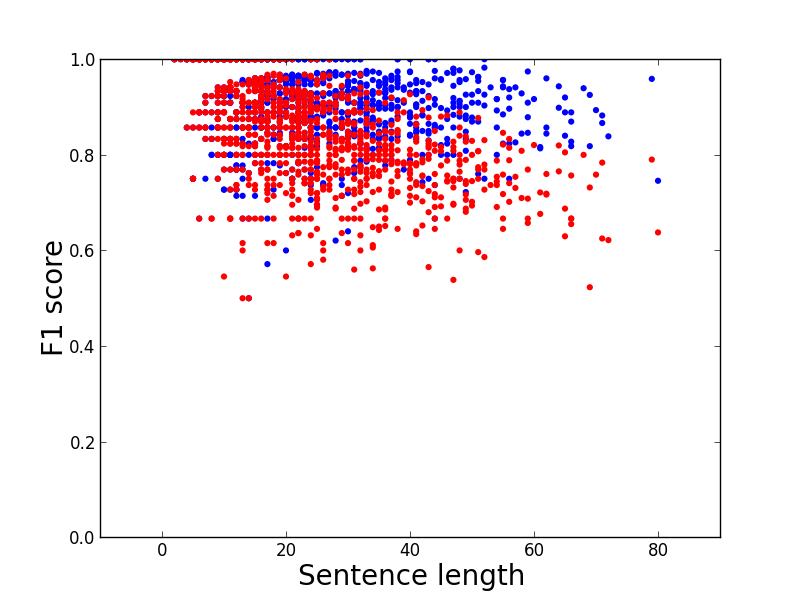
\includegraphics[keepaspectratio=true, scale = 0.35]{graph.png}}
\caption{Plot of F1 scores against sentence length. The blue dots denote the original IBM Model 1, while the red dots denote our extension.}
  \label{fig:features}
\end{figure}

\section{Conclusion}
\label{Concl}
Despite its structural limitations, such as ignoring positions of words inside sentences or the context surrounding them,
IBM Model 1 is still able to achieve good results which make it useful in machine translation tasks.

% however it makes naive assumptions by ignoring the context around a word. Estimating the translation probabilities between words with the EM algorithm


\begin{thebibliography}{}
%\bibitem[\protect\citename{Gusfield}1997]{Gusfield:97}
%Dan Gusfield.
%\newblock 1997.
%\newblock {\em Algorithms on Strings, Trees and Sequences}.
%\newblock Cambridge University Press, Cambridge, UK.

\bibitem[1]{Koehn:2010}
Philipp Koehn
\newblock 2010.
\newblock {\em Statistical Machine Translation}.
\newblock Cambridge University Press.

\bibitem[2]{Brown:2010}
Brown, Peter F and Pietra, Vincent J Della and Pietra, Stephen A Della and Mercer, Robert L
\newblock 1993.
\newblock {\em The mathematics of statistical machine translation: Parameter estimation}.
\newblock Computational linguistics.% 19.2: 263-311.

\bibitem[3]{Moore:2004}
Moore, Robert C.
\newblock 2004
\newblock {\em Improving IBM word-alignment model 1}.
\newblock Association for Computational Linguistics.

\end{thebibliography}

\appendix
\section{Translation Table}
\begin{table}[h]
\begin{tabular}{l r r}

		&Trained:	&Viterbi:\\\hline\hline
NULL &&\\\hline
.		&0.81		&0.9\\
het		&0.12		&0.05\\\
de		&0.067	&0.05\\
eigenlijke	&0.012	&0\\
onttrokken	&0.012	&0\\
aan		&3.39e-07	&0\\
significante	&3.96e-08	&0\\
meren		&3.96e-08	&0\\
territoriale	&3.96e-08	&0\\
verbod	&3.96e-08	&0\\\hline\hline
%
the&&\\\hline		
de		&0.80		&0.97\\
transparantie &0.64	&0\\
het		&0.16		&0.03\\
eigenlijke	&0.10		&0\\
onttrokken	&0.10		&0\\
van		&0.04		&0\\
re\"ele	&0.01		&0\\
territoriale	&0.00		&0\\
significante	&0.00		&0\\
meren		&0.00		&0\\\hline\hline
%
in	&&\\\hline
in				&0.64	&0.94\\
de				&0.17	&0.02\\
onderhoud			&0.12	&0.00\\
zeewaardigheidsattesten	&0.12	&0.00\\
afleveren			&0.12	&0.00\\
er				&0.08	&0.03\\
van				&0.07	&0.00\\
op				&0.03	&0\\
significante			&0.02	&0\\
meren				&0.02	&0\\\hline\hline
\end{tabular}
\caption{The top 10 scoring translations according to the training, and corresponding Viterbi probabilities.}
\label{firstPart}
\end{table}

\begin{table}[h]
\begin{tabular}{l r r}
&Trained:	&Viterbi:\\\hline\hline
.&&\\\hline
.		&0.85		&0.99\\
het		&0.15		&0.01\\
eigenlijke	&0.01 	&0\\
onttrokken	&0.01		&0\\
de		&0.01		&0\\
aan		&2.24e-07	&0\\
is		&6.72e-08	&0\\
significante	&4.43e-08	&0\\
meren		&4.43e-08	&0\\
territoriale	&4.43e-08	&0\\\hline\hline
%
all&&\\\hline
alle		&0.55	&0.79\\
duidelijke	&0.36	&0.05\\
moeten	&0.22	&0.13\\
termijn	&0.08	&0\\
een		&0.06	&0\\
en		&0.06	&0.003\\
begeven	&0.05	&0\\
re\"ele	&0.05	&0\\
die		&0.05	&0\\
leiden		&0.04	&0\\\hline\hline
%
public	&&\\\\hline
en			&0.23		&0.5\\
zo			&0.17		&0.5\\
met			&0.15		&0\\
transparante		&0.13		&0\\
komen			&0.13		&0\\
onafhankelijke	&0.10		&0\\
opinie			&0.10		&0\\
concrete		&0.08		&0\\
echter			&0.08		&0\\
keer			&0.08		&0\\
%
%should	Trained:	Viterbi:
%moeten	0.345341811231	0.5
%moet	0.326959543723	0.392857142857
%wordt	0.129993708283	0.0178571428571
%,	0.128878290535	0.0178571428571
%dat	0.121058042401	0.0357142857143
%allereerst	0.086463755169	0.0178571428571
%eveneens	0.0691683819178	0
%slachtoffer	0.0687902672564	0.0178571428571
%Parlementslid	0.0592905040574	0
%geworden	0.0591591378846	0
\end{tabular}
\caption{Continuation of Table \ref{firstPart}. Same caption.}
\end{table}




\end{document}
